% !TeX program = pdflatex
\documentclass[tikz,border=8pt]{standalone}
\usepackage{tikz}
\usetikzlibrary{calc,intersections,decorations.pathreplacing,positioning}
\definecolor{FigureBlue}{HTML}{2563EB}
\definecolor{FigureOrange}{HTML}{EA580C}
\definecolor{FigureSlate}{HTML}{64748B}
\begin{document}
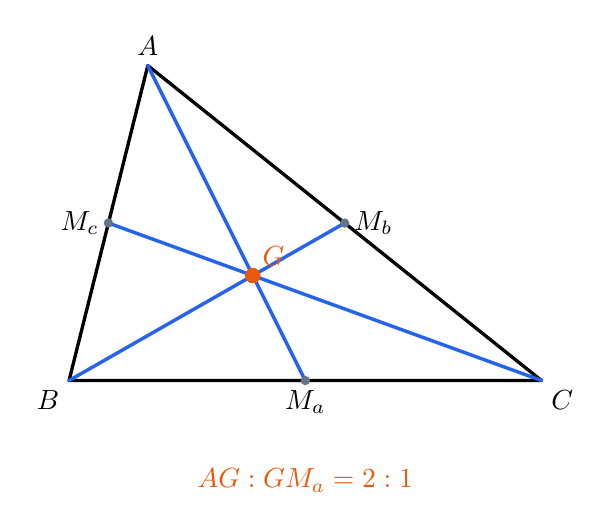
\begin{tikzpicture}[line cap=round,line join=round]
  \coordinate (A) at (1,4);
  \coordinate (B) at (0,0);
  \coordinate (C) at (6,0);
  \coordinate (Ma) at ($(B)!.5!(C)$);
  \coordinate (Mb) at ($(C)!.5!(A)$);
  \coordinate (Mc) at ($(A)!.5!(B)$);
  \path[name path=medianA] (A)--(Ma);
  \path[name path=medianB] (B)--(Mb);
  \path[name intersections={of=medianA and medianB,by=G}];
  \draw[line width=1.2pt] (A)--(B)--(C)--cycle;
  \draw[FigureBlue,line width=1.25pt] (A)--(Ma) (B)--(Mb) (C)--(Mc);
  \foreach \P in {Ma,Mb,Mc}{\fill[FigureSlate] (\P) circle (1.7pt);}
  \fill[FigureOrange] (G) circle (2.8pt);
  \node[above] at (A) {$A$};
  \node[below left] at (B) {$B$};
  \node[below right] at (C) {$C$};
  \node[below] at (Ma) {$M_a$};
  \node[right] at (Mb) {$M_b$};
  \node[left] at (Mc) {$M_c$};
  \node[above right,text=FigureOrange] at (G) {$G$};
  \node[below=10mm,text=FigureOrange] at (Ma) {$AG:GM_a=2:1$};
\end{tikzpicture}
\end{document}
